\section{Setup}
Follow this guide to have a Development Environment for Linux and Windows. You have to download Eclipse and CMake. Windows users can use MinGW as a C/C++ compiler. 

\subsection{Eclipse with CDT (Windows/Linux)}
Eclipse is an Integrated Development Environment (IDE). It is possibly best known as a Java development platform, but can be extended for languages such as C/C++, PHP, Python and more. The easiest way to get Eclipse with C/C++ support is to download \textit{Eclipse for C++ Developers} for your operating system at: \url{http://www.eclipse.org/downloads/}. The download already includes the CDT Plugin (C/C++ Development Toolkit).

There is no installation. Just unpack and start the eclipse executable.

\subsection{MinGW (Windows only)}
This step is Windows only. \htmladdnormallink{MinGW (Minimalist GNU for Windows)}{http://www.mingw.org} is a port of the \htmladdnormallink{GNU Compiler Collection (GCC)}{http://gcc.gnu.org} and can be used for development of native \htmladdnormallink{Microsoft Windows}{http://www.microsoft.com/windows} applications. Download the automated mingw-get-installer \htmladdnormallink{from sourceforge}{http://sourceforge.net/projects/mingw/files/Automated\%20MinGW\%20Installer/mingw-get-inst/} (called \textit{mingw-get-inst-20101030.exe} at time of writing this). If the path to the download changes, navigate there from the MinGW project page at: \url{http://www.mingw.org}. Be sure to select \textit{"C++ Compiler"} in the \textit{Compiler Suite} dialog during setup.

MinGW doesn't add its binaries to the global Windows PATH environment. The MinGW Page says: \textit{Add }\verb|C:\MinGW\bin;|\textit{ to the PATH environment variable by opening the System control panel, going to the Advanced tab, and clicking the Environment Variables button. If you currently have a Command Prompt window open, it will not recognize the change to the environment variables; you will need to open a new Command Prompt window to get the new PATH.}

\subsection{CMake}
\htmladdnormallink{CMake}{http://www.cmake.org} is an open-source, cross-platform build system used by many opensource projects including: \htmladdnormallink{OpenCV}{http://opencv.willowgarage.com}, \htmladdnormallink{MiKTeX}{http://www.miktex.org} or \htmladdnormallink{Blender 3D}{http://www.blender.org}. It works on Linux, Windows, Mac OS X and can generate (among many others) Eclipse CDT project files and that's why it is suggested as a build system for OpenCV projects.

\subsubsection*{Windows} 
Download the installer from the \htmladdnormallink{Resources Page}{http://www.cmake.org/cmake/resources/software.html} at \url{http://www.cmake.org} (called cmake-2.8.3-win32-x86.exe at time of writing). This will install cmake, ccmake and the cmake-gui.

Make sure to select \textit{"Add CMake to the system PATH for all users"} during setup.

\subsubsection*{Linux}
CMake is often available from a distributions repository or can be downloaded as an installer from the \htmladdnormallink{Resources Page}{http://www.cmake.org/cmake/resources/software.html} at \url{http://www.cmake.org}. Installing the generic Linux binaries with the is done by typing:
\begin{lstlisting}
sudo sh cmake-2.8.3-Linux-i386.sh --prefix=/usr/local 
\end{lstlisting}

In Debian or Ubuntu cmake can be installed with apt:
\begin{lstlisting}
sudo apt-get install cmake cmake-gui
\end{lstlisting}


\subsection{OpenCV}
\htmladdnormallink{OpenCV}{http://opencv.willowgarage.com} is a Computer Vision Library started by \htmladdnormallink{Intel}{http://www.intel.com} in 1999 and now actively developed by \htmladdnormallink{Willow Garage}{http://www.willowgarage.com}. It includes advanced computer vision algorithms and sets the focus on real-time image processing. In 2009 OpenCV2 got a C++ interface and integrates with Python. If you encounter any problems with this install guide consult the \htmladdnormallink{OpenCV Install Guide}{http://opencv.willowgarage.com/wiki/InstallGuide} aswell.
 
\subsubsection*{Windows}
\htmladdnormallink{Mircosoft Windows}{http://www.microsoft.com/windows} users download the Windows installer from the sourceforge repository of OpenCV at \url{http://sourceforge.net/projects/opencvlibrary/}. (called \htmladdnormallink{OpenCV-2.2.0-win32-vs2010.exe}{http://sourceforge.net/projects/opencvlibrary/files/opencv-win/2.2/} at time of writing this). 

Make sure to select \textit{"Add OpenCV to the system PATH for all users"} during setup.

\subsubsection*{Linux}
Linux users should inspect their repositories, because most distributions have pre-packaged binaries. In Debian/Ubuntu you simply type:
\begin{lstlisting}
sudo apt-get install opencv opencv-doc
\end{lstlisting}

\subsubsection*{Build OpenCV from sources}
OpenCV is open source and comes with CMake as build system. Sometimes you need to compile OpenCV yourself, for example if the pre-packaged binaries use SSE2 and your CPU doesn't support SSE2. If so, download the OpenCV sources, unpack them and cd to the directory.

For building OpenCV from source type:
\begin{lstlisting}
cmake .
make 
sudo make install
\end{lstlisting}

\subsubsection*{Building OpenCV without SSE2}
If you are actually working on a CPU without SSE2 you will need to deselect the SSE2 build option before compiling it, otherwise OpenCV won't work as expected. To see which flags your CPU supports (assuming Linux), type \lstinline{cat /proc/cpuinfo | grep flags} in a terminal.

On my workstation:

\begin{lstlisting}
philipp@banana:~$ cat /proc/cpuinfo | grep flags
flags           : fpu vme de pse tsc msr pae mce cx8 sep mtrr pge mca cmov pat pse36 mmx fxsr sse syscall mp mmxext 3dnowext 3dnow up ts fid vid
\end{lstlisting}

It's an \htmladdnormallink{AMD}{http://www.amd.com} Athlon XP and does not support SSE2. In order to turn off SSE2 support for OpenCV with the cmake-gui:
\begin{itemize}
\item Start \texttt{cmake-gui} either from prompt or menu.
\item Set the OpenCV source folder as \textit{Source Directory} and \textit{Build Directory}
\item Click \textit{configure} and choose: \texttt{Unix Makefiles}.
\item Deselect \textit{ENABLE\_SSE2} support from the list of flags.
\item Click \textit{configure} again to accept the setup.
\item Click \textit{generate} and proceed with the normal compiling procedure as described above.
\end{itemize}

The command line for doing the same would be (assuming you are in the OpenCV folder):

\begin{lstlisting}
cmake -DENABLE_SSE2=OFF .
\end{lstlisting}
followed by:
\begin{lstlisting}
make
sudo make install
\end{lstlisting}


% 
% \section{Getting started with CMake}
% This chapter serves as an introduction to CMake, because it is used for the OpenCV project. Instead of making up a simple Hello World, it will show how to write, test and build a library with CMake and the \htmladdnormallink{Boost Framework}{http://www.boost.org}.
% \subsection*{Problem}
% Imagine your are working on a project with GPS data and you are told to write and test a library, let's call it \textit{geolib}, to calculate the distance between two positions on earth (also called great-circle distance or orthodromic distance). Points on earth are given in latitude ($\phi$) and longitude ($\lambda$) and for the distance calculation one can use the haversine formula:
% \begin{equation}
% \label{eq:haversine}
% \operatorname{haversin}\left(\frac{d}{R}\right) = \operatorname{haversin}(\varphi_2 - \varphi_1) + \cos(\varphi_1) \cos(\varphi_2)\,\operatorname{haversin}(\Delta\lambda).
% \end{equation}
% 
% Where $haversin$ is:
% 
% \begin{displaymath}
% haversin(\theta) = \sin^2 (\theta / 2)
% \end{displaymath}
% 
% And applying the inverse haversine gives the distance $d$:
% 
% \begin{displaymath}
% d = R \, \operatorname{haversin}^{-1}(h) = 2 R \arcsin\left(\sqrt{h}\,\right)
% \end{displaymath}
%  
% Where $h$ is:
% \begin{displaymath}
% h =  \operatorname{haversin}(\frac{d}{R})
% \end{displaymath}
% 
% \subsection*{Files}
% The final project has a structure shown in Listing \ref{lst:cmake_files}. The source files are in the appendix or can be downloaded from: \url{http://bytefish.de/lib/exe/fetch.php?media=blog:cmake_example.zip}.
% 
% \begin{lstlisting}[label=lst:cmake_files, caption=Project structure.]
% philipp@banana:~/git/cmake$ tree src
% src/
% |-- CMakeLists.txt
% |-- geolib
% |   |-- geolib.cc
% |   |-- geolib.h
% |   `-- test.cc
% `-- main.cc
% 
% 1 directory, 5 files
% \end{lstlisting}
% 
% 
% \subsection*{Implementation}
% 
% You start by implementing the library. The header file in Listing \ref{lst:geolib.h} is using \htmladdnormallink{Doxygen}{http://www.stack.nl/~dimitri/doxygen/} annotations to document the code. Doxygen is not introduced here, but it is strongly advised to document your work (because someone wants to \textit{use} and \textit{understand} it aswell). The corresponding source file in Listing \ref{geolib.cc} implements the haversine formula given in equation \ref{eq:haversine}.
% 
% \begin{lstlisting}[language=C++, label=lst:geolib.h, caption=lst:geolib.h]
% #ifndef _geolib_h
% #define _geolib_h
% #include <math.h>
%  
% /**
% * @author philipp
% * @date 2010
% */
% namespace geolib {
%  
%     const double DEG2RAD = M_PI / 180.0;
%     const double RAD2DEG = 180.0 / M_PI;
%     const double EARTH_RADIUS = 6371.01;
%  
%     /**
%      * @brief great-circle distance (shortest distance between two points on earth)
%      * @param[in] latitude point 1
%      * @param[in] longitude point 1
%      * @param[in] latitude point 2
%      * @param[in] longitude point 2
%      * @return great-circle distance
%     */
%     double great_circle_distance(double lat1, double long1, double lat2, double long2);
%  
% }
%  
% #endif
% \end{lstlisting}
% The corresponding source file in geolib.cc implements the haversine formula given in the projects description: 
% \begin{lstlisting}[language=C++, label=lst:geometry.cc, caption=geometry.cc]
% #include "geolib.h"
%  
% namespace geolib {
%  
%     double great_circle_distance(double lat1, double long1, double lat2, double long2) {
%         lat1 *= DEG2RAD;
%         long1 *= DEG2RAD;
%         lat2 *= DEG2RAD;
%         long2 *= DEG2RAD;
%  
%         double deltaLat = lat1-lat2;
%         double deltaLong = long1-long2;
%         double a = pow(sin(deltaLat/2.0),2.0) + cos(lat1) * cos(lat2) * pow(sin(deltaLong/2.0),2.0);
%         double c = 2 * asin(sqrt(a));
%  
%         return EARTH_RADIUS * c;
%     }
%  
% }
% \end{lstlisting}
% 
% \subsection{Tests}
% Software has bugs. So tests are important in software development to ensure that components are working correctly. They are a sort of living documentation and should reduce defects and failures, especially when refactoring software. If you are used to JUnit you will find the Boost unit testing framework for C++ pleasing. Boost (\url{http://www.boost.org}) is a great library that adds enormous extra power to C++.
% 
% The Boost testing framework is a set of macros to validate expressions and each macro belongs to one of the three warning levels:
% \begin{itemize}
%  \item \textbf{WARN} logs a warning if the test fails
%  \item \textbf{CHECK} continues the test on failure
%  \item \textbf{REQUIRE} stops the test on failure
% \end{itemize}
% 
% The best introduction is probably given by \htmladdnormallink{IBM developerWorks: Get to know the Boost unit test framework}{http://www.ibm.com/developerworks/aix/library/au-ctools1_boost/}. A list of available macros is given by the \htmladdnormallink{Boost documentation on testing tools}{http://www.boost.org/doc/libs/1_45_0/libs/test/doc/html/utf/testing-tools/reference.html}
% Listing \ref{lst:test.cc} shows how to test the great-circle distance of the geolib with the Boost unit testing framework. As test data I use the airport example from the Wikipedia Page on Great-circle distance: 
% 
% \begin{lstlisting}[language=C++, label=lst:test.cc, caption=test.cc]
% #define BOOST_TEST_DYN_LINK
% #define BOOST_TEST_MODULE "GeoLib Tests"
% #include <boost/test/unit_test.hpp>
% #include "geolib.h"
% 
% BOOST_AUTO_TEST_CASE(gcircle_test) {
% 
% 	double expected = 2886.448973436;
% 
% 	double bna_lat = 36.12;
% 	double bna_long = -86.67;
% 	double lax_lat = 33.94;
% 	double lax_long = -118.40;
% 
% 	double actual = geolib::great_circle_distance(bna_lat, bna_long, lax_lat, lax_long);
% 	BOOST_CHECK_CLOSE(expected, actual, 1e-5);
% 
% }
% 
% \end{lstlisting}
% 
% 
% \subsection{CMakeLists.txt: Putting it all together}
% CMake searches for a file called \textit{CMakeLists.txt} in a given directory. The CMakeLists.txt for this project is: 
% 
% \begin{lstlisting}[label=lst:CMakeLists.txt, caption=CMakeLists.txt]
% CMAKE_MINIMUM_REQUIRED( VERSION 2.6 )
% PROJECT(HELLOWORLD_PROJECT)
% INCLUDE_DIRECTORIES("${CMAKE_SOURCE_DIR}/geolib")
% ADD_LIBRARY(geolib geolib/geolib.cc geolib/geolib.h)
% ADD_EXECUTABLE(helloworld main.cc)
% TARGET_LINK_LIBRARIES(helloworld geolib)
% 
% # Tests
% FIND_PACKAGE( Boost REQUIRED COMPONENTS unit_test_framework)
% INCLUDE_DIRECTORIES(${Boost_INCLUDE_DIRS})
% ADD_EXECUTABLE(test_geolib geolib/test.cc)
% TARGET_LINK_LIBRARIES(test_geolib ${Boost_LIBRARIES} geolib)
% \end{lstlisting}
% 
% \subsection{Build}
% Building the project can be done by an out of source build: 
% \begin{lstlisting}
% philipp@banana:~/git/cmake$ mkdir build && cd build
% philipp@banana:~/git/cmake/build$ cmake ../src/
% philipp@banana:~/git/cmake/build$ make
% \end{lstlisting}
% Running the executable \textit{helloworld} calculates the distance from Berlin to Munich (in km):
% \begin{lstlisting}
% philipp@banana:~/git/cmake/build$ ./helloworld
% Distance is 508.978.
% \end{lstlisting}
% Running the test returns no errors:
% \begin{lstlisting}
% philipp@banana:~/git/cmake/build$ ./test_geolib
% Running 1 test case...
% 
% *** No errors detected
% \end{lstlisting}

\section{Getting Started with OpenCV}
Now that Eclipse, MinGW (Windows), CMake and OpenCV are installed it is time to create the first OpenCV project. It is called \textit{hello\_opencv}. Files for this example are put in a folder at: \verb|C:\workspace\hello_opencv|. Of course any valid path can be chosen and kept consistent with the example.

\subsubsection*{1. CMakeLists.txt}
CMake searches for a file called CMakeLists.txt The OpenCV library is linked against the executable. Save CMakeLists.txt from Listing \ref{lst:cmakelists.txt} to \verb|C:\workspace\hello_opencv|.
 
\begin{lstlisting}[caption=CMakeLists.txt, label=lst:cmakelists.txt]
cmake_minimum_required(VERSION 2.6)
PROJECT(hello_opencv_proj)
FIND_PACKAGE( OpenCV REQUIRED )
ADD_EXECUTABLE( hello_opencv main.cpp)
TARGET_LINK_LIBRARIES( hello_opencv ${OpenCV_LIBS} )
\end{lstlisting}

\subsubsection*{2. main.cpp}
Now the OpenCV C++ API is introduced.

\begin{lstlisting}[language=C++, label=lst:main.cpp]
#include "cv.h"
#include "ml.h"

using namespace std;

int main() {
	cv::Mat plot(240,320,CV_8UC3);
	plot.setTo(cv::Scalar(255,255,255));
	cv::putText(plot,"Hello OpenCV",Point(1,100), FONT_HERSHEY_SIMPLEX, 1.0 ,Scalar(0,0,0), 1, 8, false);
	cv::namedWindow("Hello OpenCV", CV_WINDOW_AUTOSIZE);
	cv::imshow("Hello OpenCV", plot);
	cv::waitKey();
}
\end{lstlisting}

Save main.cpp from Listing \ref{lst:main.cpp} to \verb|C:\workspace\hello_opencv|.

\subsubsection*{3. Generate project and makefiles}
We will need to import the project to eclipse, so we generate the CDT specific Makefiles:

\begin{itemize}
\item Start the \textit{cmake-gui}
\item Browse to \verb|C:\workspace\hello_opencv| as \textit{Source Folder} and \textit{Build Folder}
\item Click \textit{configure} and select "Eclipse CDT4 - Unix Makefiles" from the Dialog
\item Click \textit{configure} again to accept the configuration
\item Click \textit{generate} to generate the Makefiles and Eclipse related project files
\end{itemize}

Your folder will now look like this:

\begin{lstlisting}
C:\workspace\hello_opencv>dir

11.12.2010  14:33    <DIR>          .
11.12.2010  14:33    <DIR>          ..
11.12.2010  14:33            22.202 .cproject
11.12.2010  14:33             3.591 .project
11.12.2010  14:28            29.062 CMakeCache.txt
11.12.2010  14:33    <DIR>          CMakeFiles
11.12.2010  14:18               190 CMakeLists.txt
11.12.2010  14:28             1.470 cmake_install.cmake
11.12.2010  14:14               556 main.cpp
11.12.2010  14:33             5.179 Makefile
\end{lstlisting}

If you feel more familiar with a terminal type:

\begin{lstlisting}
C:\> cd C:\workspace\hello_opencv
C:\> cmake -G"Eclipse CDT4 - Unix Makefiles" .
\end{lstlisting}

\subsubsection*{4. Import project and makefiles into Eclipse}
Start Eclipse and from the menu choose:
\begin{enumerate}
 \item \verb|File -> Import...|
 \item \verb|General -> Existing Projects into Workspace|
 \item Select \verb|C:\workspace\hello_opencv| as root directory
 \item Click \verb|Finish|
\end{enumerate}

\subsubsection*{5. Build and run the project}
To build the project:
 \begin{itemize}
  \item \verb|Project -> Build All|
 \end{itemize}
To run the project:
\begin{itemize}
 \item \verb|Run -> Run|
\end{itemize}

And a window similar to Figure \ref{fig:helloworld} pops up.

\begin{figure}[ht!]
\label{fig:helloworld}
\caption{OpenCV: Hello World}
 \begin{center}
   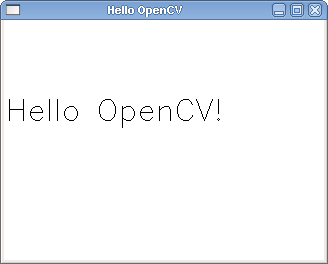
\includegraphics[scale=0.5]{img/helloopencv.png}
 \end{center}
\end{figure}